% !TeX root = sigqdyn_tr.tex
% ================================================================
\section{Scaled Sojourn Time: Details}\label{sec:scaled_sojourn_details}

% ----------------------------------------------------------------
\subsection{Scaled Sojourn Time: Analysis}\label{sec:scaled_sojourn_analysis}

\begin{figure}[h]
	\centering
	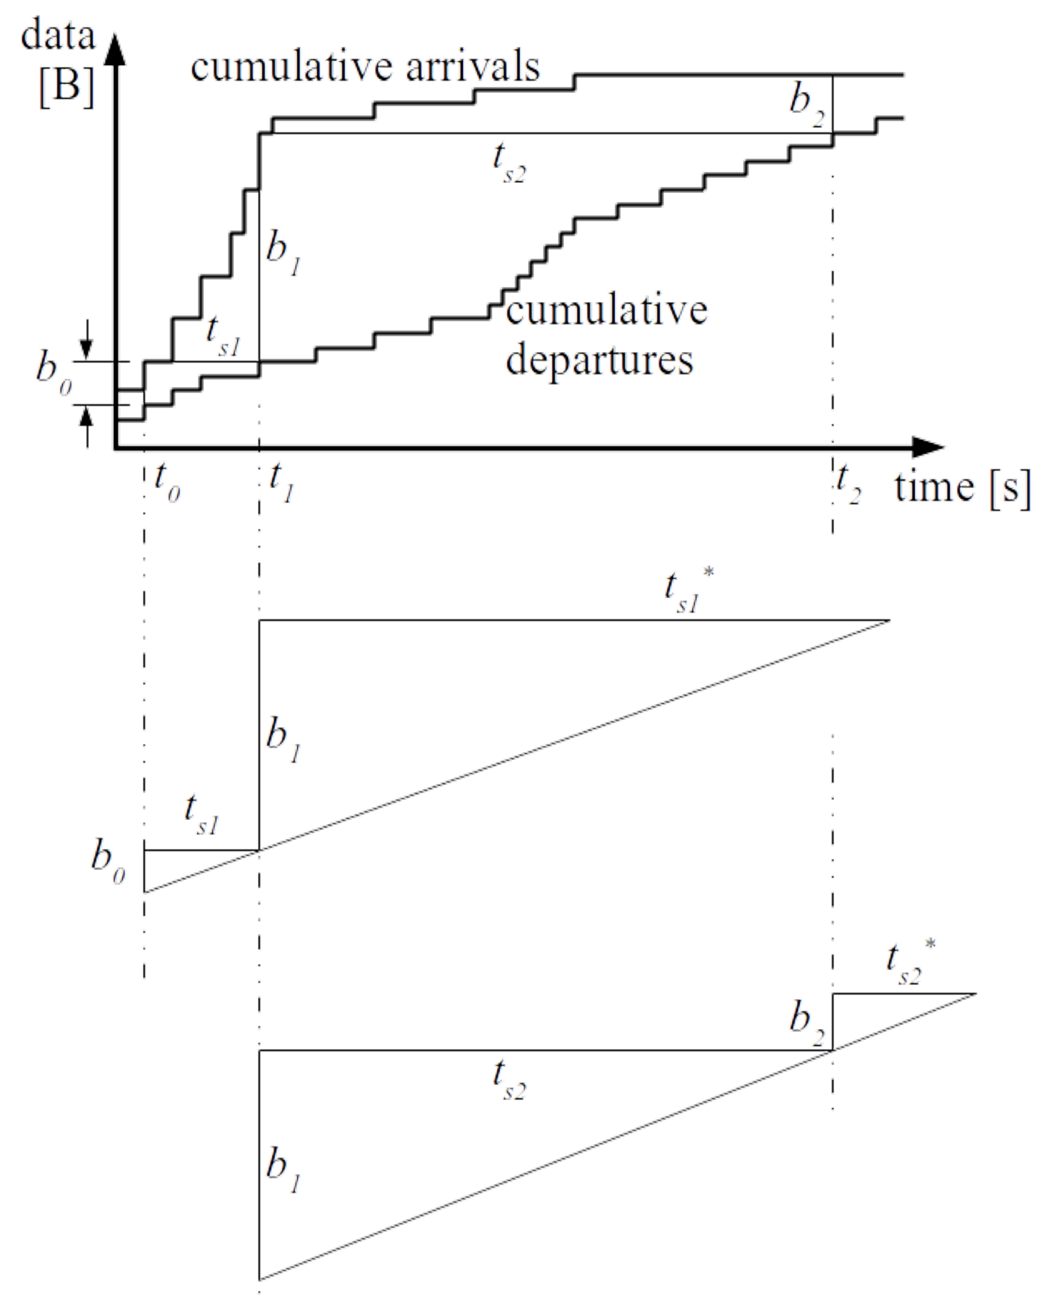
\includegraphics[width=\columnwidth]{scaled-sojourn}
	\caption{Rationale for Scaling Sojourn Time}\label{fig:scaled-sojourn}
\end{figure}

\autoref{fig:scaled-sojourn} visualizes a geometric interpretation of the rationale for scaling the sojourn time. The two plots in the chart at the top of the figure show cumulative arrivals and departures of data in packets. Between times \(t_0\) and \(t_1\) a burst of packets arrives and between \(t_1\) and \(t_2\) a few packets arrive at first, then none. Over the whole time the departure rate is varying independently as, for example, a WiFi link might. At any time, for instance \(t_1\), the sojourn time  (\(t_{s1}\)) can be visualized as the horizontal distance back from the departures plot to the arrivals plot. And the backlog is shown as the vertical distance between the plots (\(b_1\)).

It can be seen that the sojourn time (\(t_{s1}\)) between \(t_0\) and \(t_1\) takes account of the departure rate, but not the arrival rate (the burst), during that time. It is proposed to scale the sojourn time by the ratio of the backlogs at departure and arrival of the packet. That is \(t_{s1}^* = t_{s1} b_1/b_0\). This scaled sojourn time uses all the latest information available at time \(t_1\). 

The schematic in the middle of the figure shows, using similar triangles, how scaled sojourn time is constructed.  The departure rate during the sojourn is represented by the slope of the smaller of the middle triangles. The larger triangle extrapolates that departure rate to predict the time (\(t_{s1}^*\)) that it will take for the most recent backlog to drain.

The lower schematic shows the situation at time \(t_2\). The actual sojourn time of the new head packet \(t_{s2}\) is slightly shorter than the prediction \(t_{s1}^*\). From this new actual sojourn time, a new prediction can now be constructed  from the slightly steeper rate slope. This time the backlog \(b_2\) has reduced  during the sojourn of the head packet, because there has been a lull in arrivals since \(t_1\). Therefore the formula predicts that the sojourn time will be scaled down relative to its measured value.

We will now return to time \(t_1\) and derive the scaled sojourn time algebraically, rather than geometrically. The departure rate during the sojourn of the head packet is
\begin{align}
	r_{d1} &= \frac{b_0}{t_{s1}}.\label{eqn:drate}
\intertext{The expected service time to drain the backlog at \(t_1\) is}
	t_{s1}^* &= \frac{b_1}{r_{d1}}.\notag
\intertext{Substituting from \autoref{eqn:drate}:}
				&= t_{s1} \frac{b_1}{b_0}.\label{eqn:sojourn}
\end{align}

The expected service time can also be expressed in terms of a ratio of average arrival and departure rates during the sojourn, \(r_{a1}\) and \(r_{d1}\). The backlog at \(t_1\) can be expressed in terms of the arrival rate over the sojourn time:
\begin{align}
	b_1 &= t_{s1} r_{a1}.\label{eqn:backlog}
\intertext{Substituting this into \autoref{eqn:sojourn}, the scaled sojourn time at \(t_1\),}
	t_{s1}^* &= t_{s1} \frac{r_{a1}}{r_{d1}}
\end{align}
That is, scaling the sojourn time by the ratio between the backlogs at dequeue and enqueue is equivalent to scaling it by the ratio between the average arrival and departure rates between enqueue and dequeue.

% ----------------------------------------------------------------
\subsection{Implementing Scaled Sojourn Time}\label{sec:inst_svc_time_impl}

To implement scaling of the sojourn time, it is probably easiest to store \texttt{backlog\_enq} in the packet's metadata when the packet is enqueued. Then at dequeue it can be divided into \texttt{backlog\_deq}. 

But some implementations choose not to do too much at dequeue, because there is limited time between the packet reaching the head of the queue and starting to be forwarded. Therefore, it could be challenging to measure the system time, subtract the stored timestamp then also scale the result by a ratio.

The division in the ratio can be avoided by in at least two ways:
\begin{itemize}[nosep]
	\item Multiply the threshold(s) of the AQM by \texttt{backlog\_enq} rather than dividing it into \texttt{backlog\_deq} (as in \S\,\ref{sec:time-adj_thresh});
	\item Use the techniques below to optimize execution, although efficiency will be machine-architecture-dependent, and precision is only to the nearest binary order of magnitude:
\end{itemize}

{\small\texttt{qdelay <<= (lg(backlog\_deq) - lg(backlog\_enq)\\+ 1/2)}}\\
It is roughly equivalent to multiplying by the ratio between the backlogs, to the nearest integer power of 2.

The \texttt{<<=} operator bit-shifts \texttt{qdelay} to the left by the expression on the right. \texttt{lg()} is the logarithm function base 2. The expression bit-shifts \texttt{qdelay} to the left by the difference between the logs of the backlogs at enqueue and dequeue. The addition of 1/2 is necessary so that integer truncation of the result will round to the nearest integer, rather than always rounding down. 

The \texttt{clz()} function to count leading zeros could be used as a cheaper but more approximate base-2 log function, as follows:\\
{\small\texttt{qdelay <<= (clz(backlog\_enq) - clz(backlog\_deq))}}\\
This also avoids the need for any boundary checking code.

For example, if the \texttt{backlog\_*} variables are 32-bit unsigned integers and
\begin{itemize}[nosep]
	\item[] \texttt{backlog\_enq = 3000}, so \texttt{clz(3000)=20}
	\item[] \texttt{backlog\_deq = 30000}, so \texttt{clz(30000)=17}
\end{itemize}
Then
\begin{itemize}[nosep]
	\item[] \texttt{qdelay <<= 20 - 17}
\end{itemize}
is the same as
\begin{itemize}[nosep]
    \item[] \texttt{qdelay *= 2\^{}3},\\
\end{itemize}
which scales qdelay by 8, which approximates to \texttt{30,000/3,000 = 10} but is an integer power of 2. This is sufficient to scale the sojourn time to the correct binary order of magnitude, while still taking account of all the latest information in the queue.

However, \texttt{clz()} introduces truncation bias because it always rounds down, which could lead the result to be persistently out by up to \(\times2\) or \(/2\) for a particular target sojourn time. Using the \texttt{lg()}-based expression could be out by from \(\sqrt{2}\) to \(1/\sqrt{2}\), but with no bias---it is equally likely to be out either way.

A high performance implementation will maintain the backlog of a queue by maintaining two variables (much like the two plots at the top of \autoref{fig:scaled-sojourn}):
\begin{itemize}[nosep]
	\item[] \texttt{count\_enq} written solely by the enqueue routine;
	\item[] \texttt{count\_deq} written solely by the dequeue routine
\end{itemize}	
Then the backlog can be measured as \texttt{count\_enq - count\_deq}. These two shared variables can be read from any routine, but they are only incremented by the routine that owns them, which avoids the performance hit of a mutual exclusion lock. The two counters monotonically increase like the system clock for the sojourn measurement, but at the rate of data transfer in and out respectively, not the rate of time passing. 

